\section{Trajectory planning}
\subsection{Point to point tracking}
The main objective is to follow a path so it is desirable to test the controller for a path as well. The \figref{fig:pathTS} shows how each joint manages to follow the desired path shown in \figref{fig:IKcom}. One can see that the robot lags behind the desired path. This path is only time dependent so it changes without respect to if the robot arm has managed to get the desired position or not.\\\\
\def\picsSiz{1.08}
\begin{figure*}[htbp]
    \centering
    \begin{subfigure}[htbp]{0.45\textwidth}
        \centering
        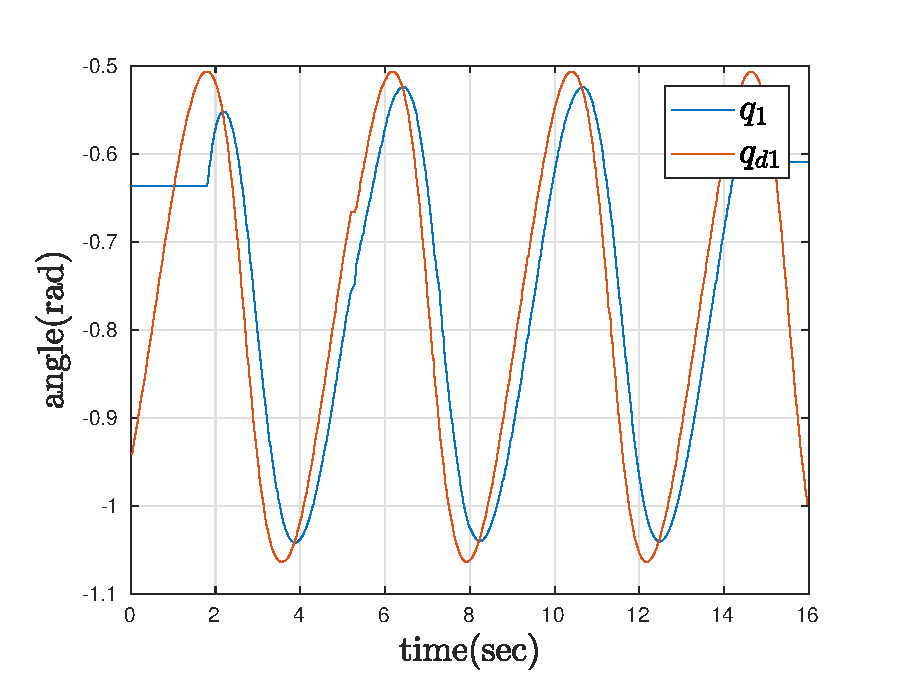
\includegraphics[width = \picsSiz\linewidth]{img/pathF1.eps}
        \caption{}
    \end{subfigure}
    ~ 
    \begin{subfigure}[htbp]{0.45\textwidth}
        \centering
        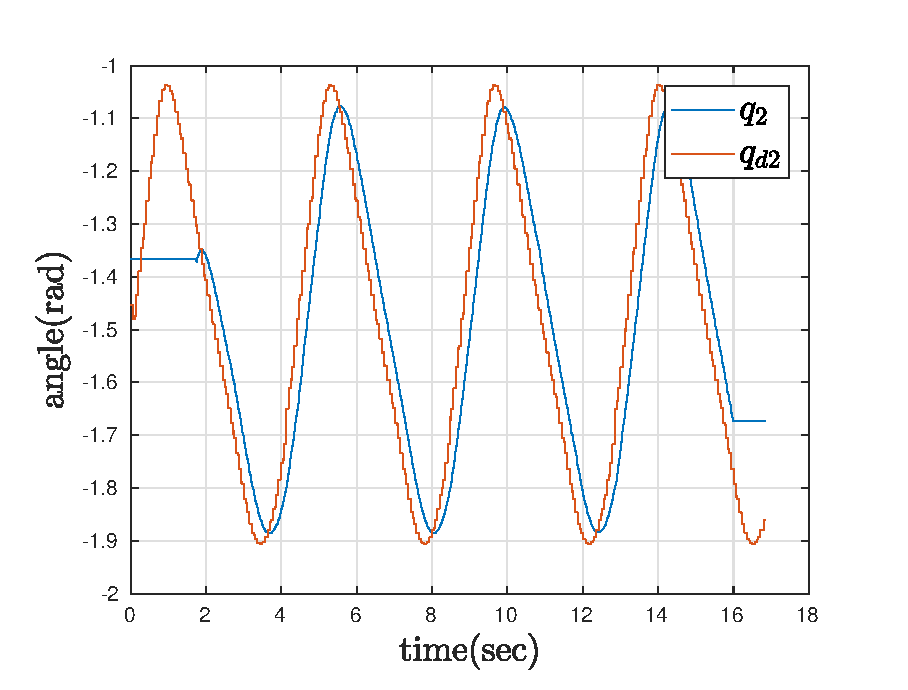
\includegraphics[width = \picsSiz\linewidth]{img/pathF2.eps}
        \caption{}
    \end{subfigure}
    ~
    \centering
    \begin{subfigure}[htbp]{0.45\textwidth}
        \centering
        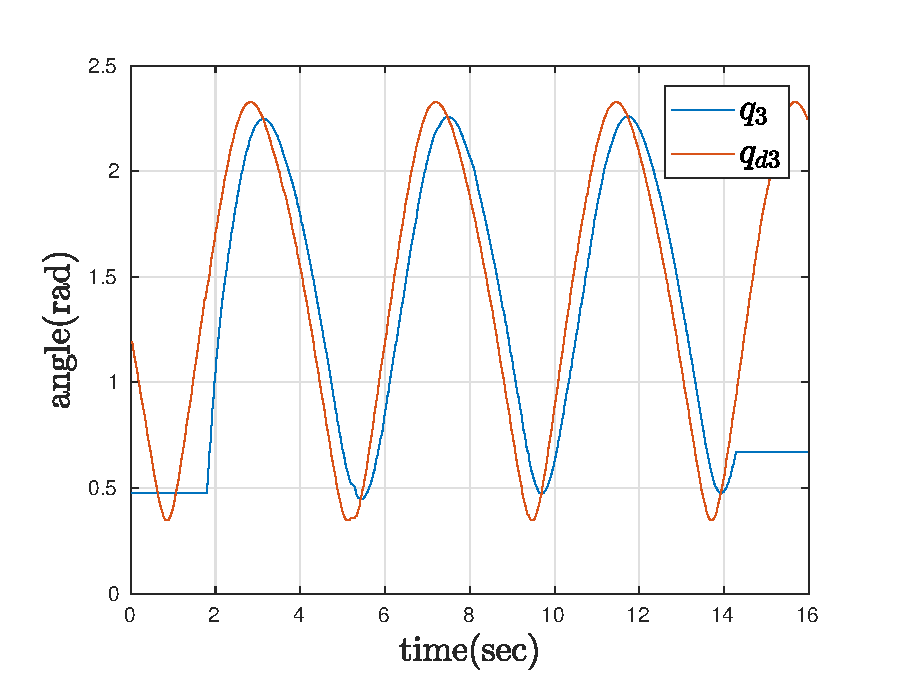
\includegraphics[width = \picsSiz\linewidth]{img/pathF3.eps}
        \caption{}
    \end{subfigure}
    ~ 
    \begin{subfigure}[htbp]{0.45\textwidth}
        \centering
        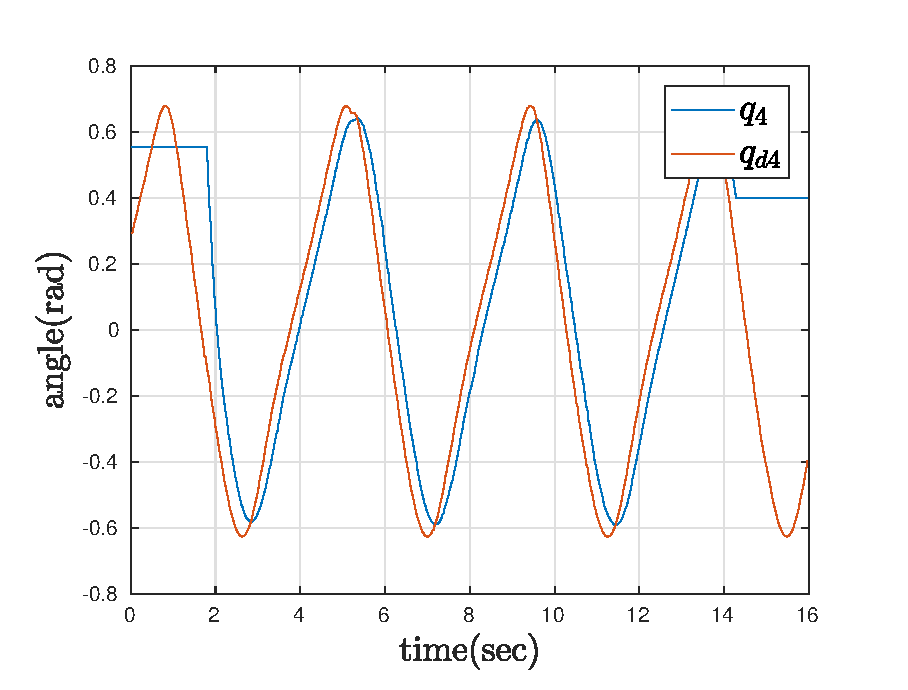
\includegraphics[width = \picsSiz\linewidth]{img/pathF4.eps}
        \caption{}
    \end{subfigure}
    ~
    \begin{subfigure}[htbp]{0.45\textwidth}
        \centering
        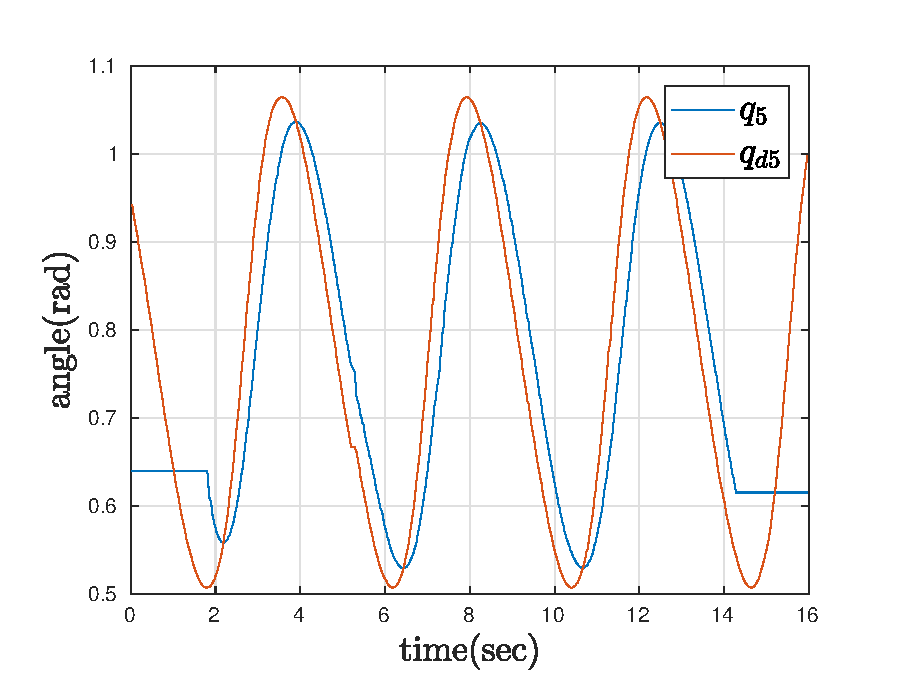
\includegraphics[width = \picsSiz\linewidth]{img/pathF5.eps}
        \caption{}
    \end{subfigure}
    \caption{Path following}
    \label{fig:pathTS}
\end{figure*}
The only information the robot gets is the point it is supposed to get to. It is therefore wanted to pass it some more information about the path. \cite{Siciliano} gives a method to use the slope of the trajectory to find the joint velocity in the trajectory
\begin{align*}
    \dot{q}_i = 
    \begin{cases}
    0\hphantom{ \frac{1}{2}(v_i+v_{i+1})}\;\;sgn(v_k)\ne sgn(v_{i+1})\\
    \frac{1}{2}(v_i+v_{i+1}) \quad  sgn(v_i)= sgn(v_{i+1})
    \end{cases}
\end{align*}
where $v_i = \frac{q_i-q_{i-1}}{t_i-t_{i-1}}$ and when you get to the last point $N$ the joint velocity $q_N$ should be zero. Since the error between the executed trajectory and the desired trajectory can be seen as a time delay one can also add the next points as a reference:
\begin{align*}
    \tilde{q} = q_{d_i}-q + \frac{q_{d_{i+1}}-q }{2}+\frac{q_{d_{i+2}}-q }{2}
\end{align*}
The results are given in \figref{fig:pathTSff}. One can see that the error is almost gone. 



\def\picsSiz{1.08}
\begin{figure*}[htbp]
    \centering
    \begin{subfigure}[htbp]{0.45\textwidth}
        \centering
        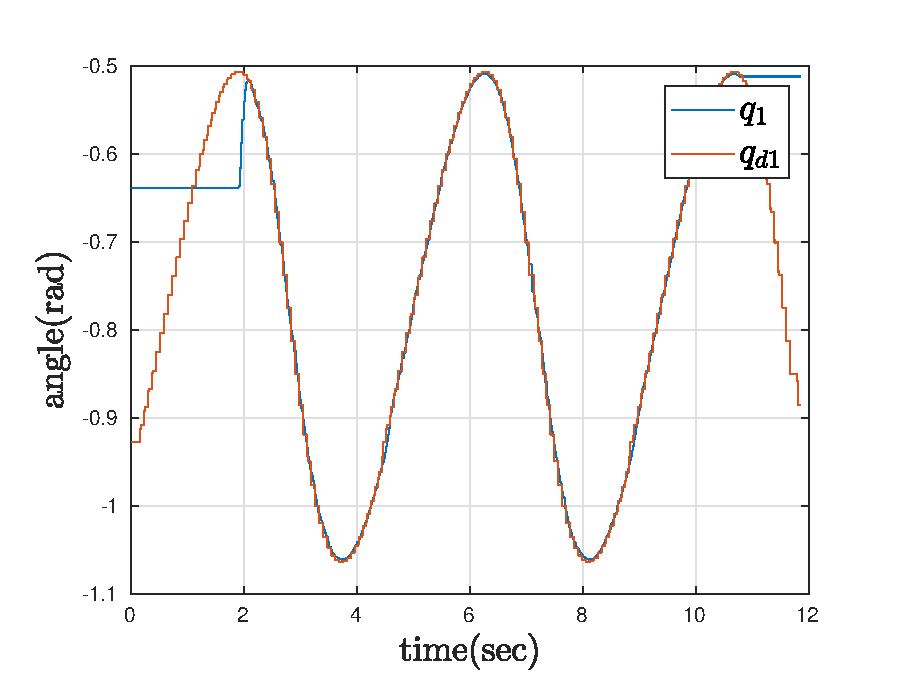
\includegraphics[width = \picsSiz\linewidth]{img/pathF1ff.eps}
        \caption{ }
    \end{subfigure}
    ~ 
    \begin{subfigure}[htbp]{0.45\textwidth}
        \centering
        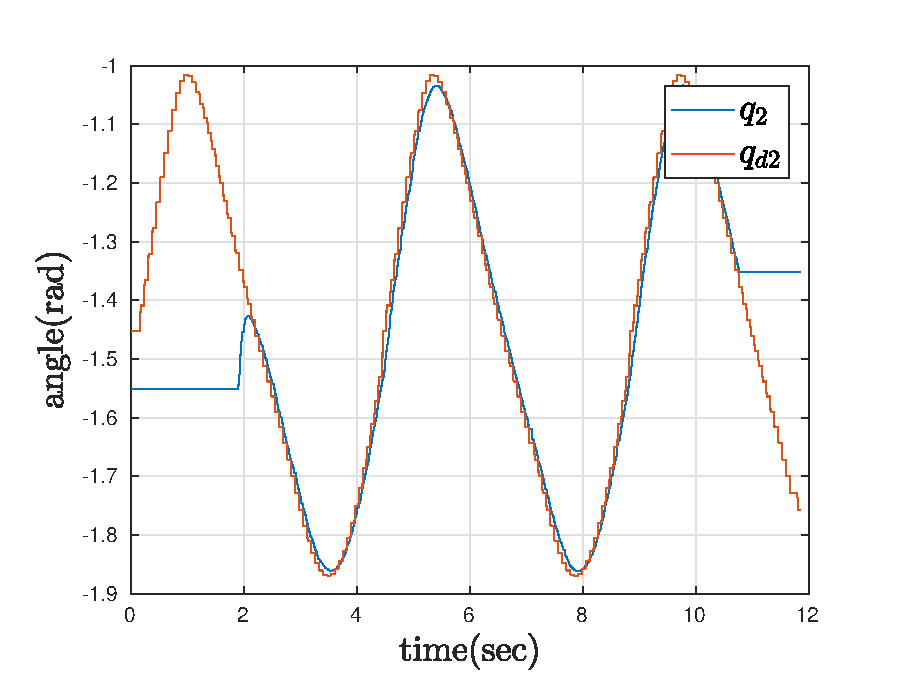
\includegraphics[width = \picsSiz\linewidth]{img/pathF2ff.eps}
        \caption{ }
    \end{subfigure}
    ~
    \centering
    \begin{subfigure}[htbp]{0.45\textwidth}
        \centering
        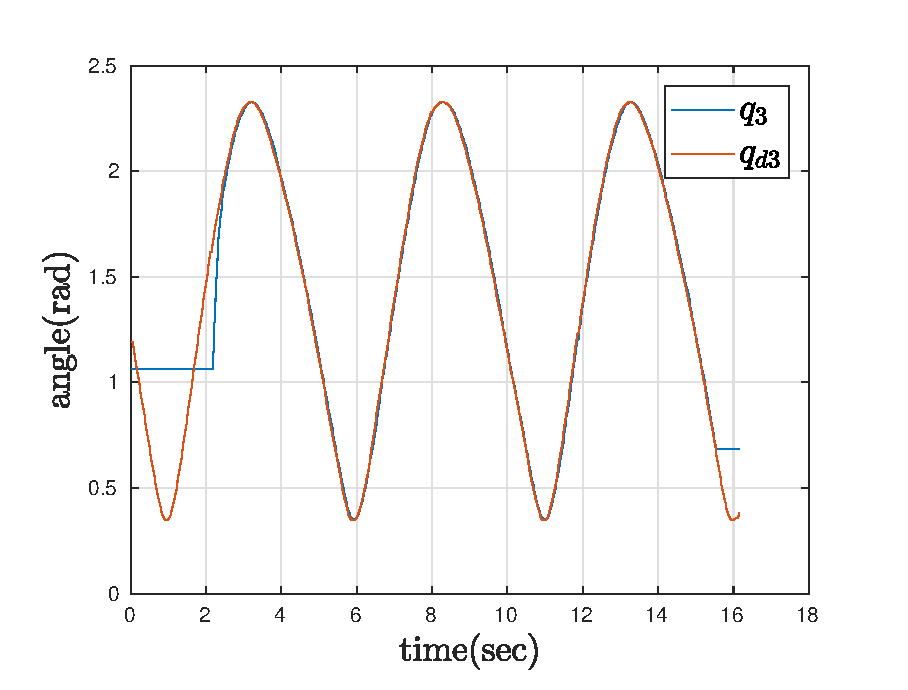
\includegraphics[width = \picsSiz\linewidth]{img/pathF3ff.eps}
        \caption{ }
    \end{subfigure}
    ~ 
    \begin{subfigure}[htbp]{0.45\textwidth}
        \centering
        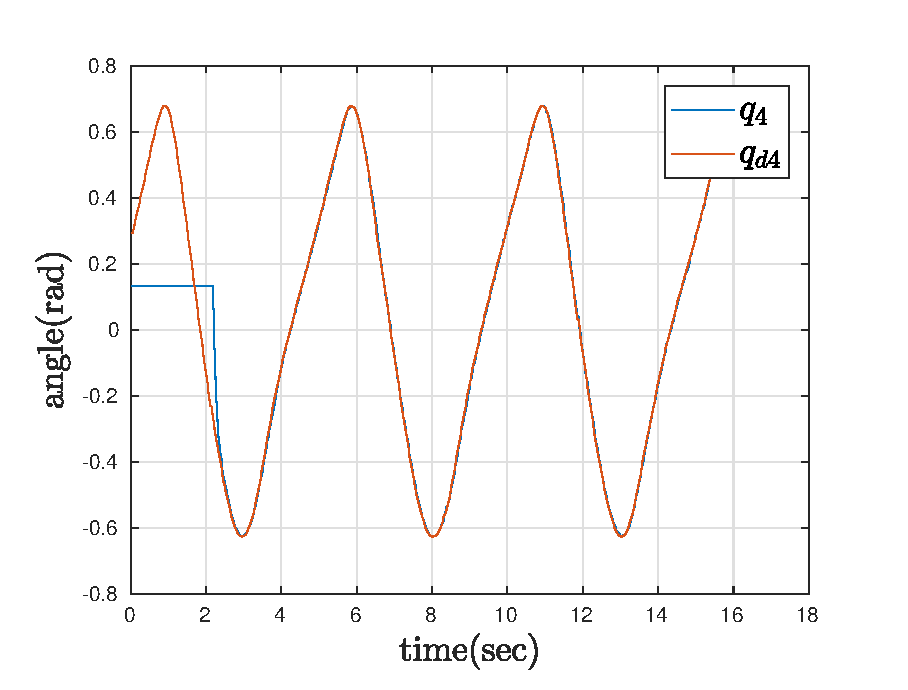
\includegraphics[width = \picsSiz\linewidth]{img/pathF4ff.eps}
        \caption{ }
    \end{subfigure}
    ~
    \begin{subfigure}[htbp]{0.45\textwidth}
        \centering
        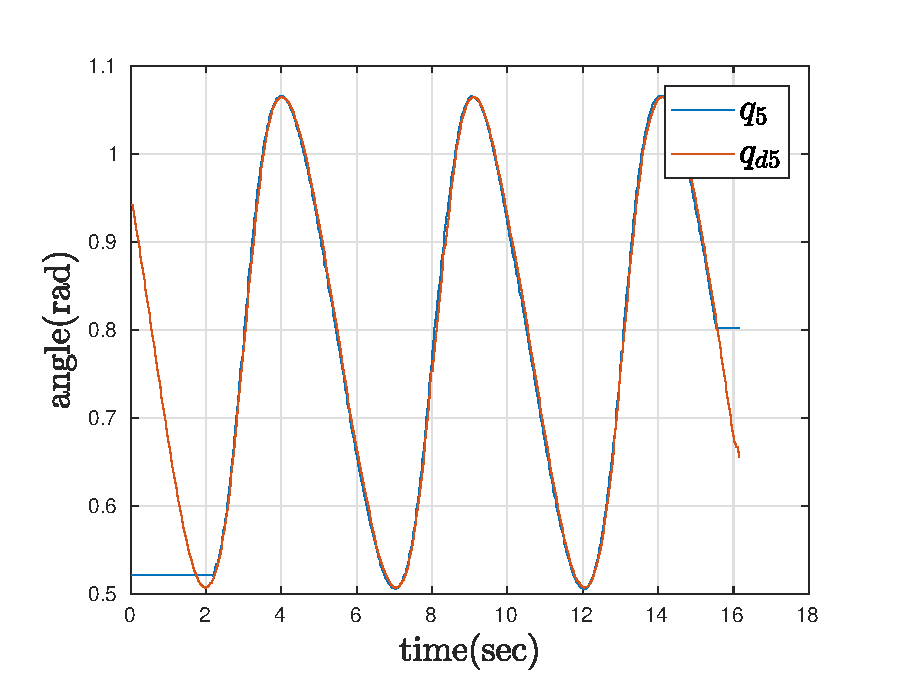
\includegraphics[width = \picsSiz\linewidth]{img/pathF5ff.eps}
        \caption{ }
    \end{subfigure}
    \caption{Path following with trajectory planner}
    \label{fig:pathTSff}
\end{figure*}


\section{Motion planning}
Until now we have just used a predefined path that has been made to test the different aspects of the manipulator. If it is wanted to go to one point to another it can be solved by creating a spline between these two points and do path following\cite{Spline}\cite{MatlabSpline}\cite{MatlabSpline2}. The task in not so easy if there are obstacles present. We then need to find a set of points such that the obstacle is avoided. One algoritgm for solving this is the \textit{rapidly-exploring random tree (RRT)} which gives good results without any parameter tuning\cite{Lavalle}. 
\subsection{Rapidly exploring Random Tree (RRT)}
The RRT algorithm is creating a space-filling tree and in our case it can be used with obstacles in the search space such that the obstacle will be an illegal object where the three cannot expand and thus using shortest path algorithm to find a path trough the tree such that we get to the desired point and avoiding the obstacle. In \figref{fig:rrt2dex} an example is given of the algorithm. An obstacle ha been placed in the search space and the wanted point is behind the obstacle relative to the origin \cite{rrt}.
\begin{figure}[htbp]
  \centering
  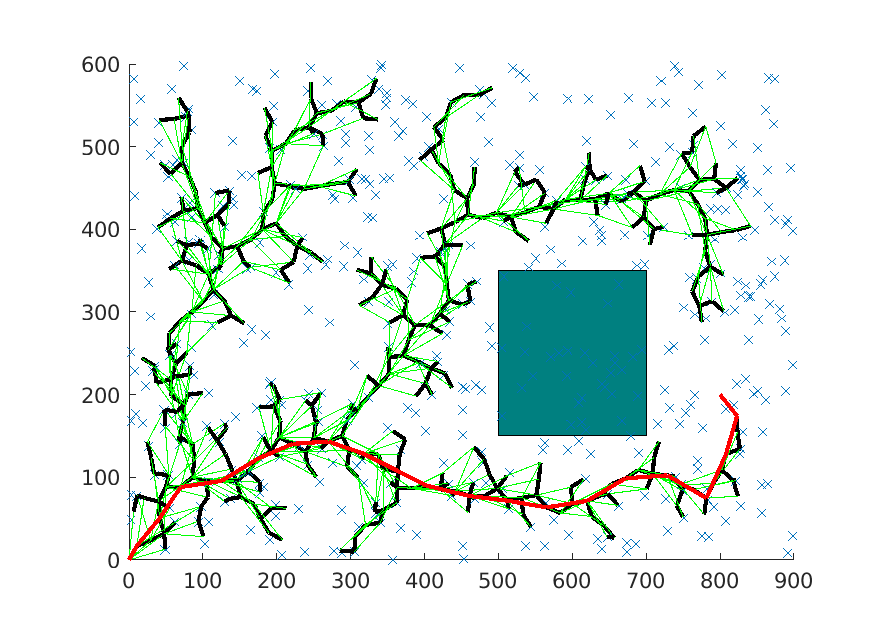
\includegraphics[width=.9\textwidth]{img/rrt2dex.eps}
  \caption{2D example of the RRT algoritm}
  \label{fig:rrt2dex}
\end{figure}
The next step is to expand this to a 3D example and do the same there. The toolbox provided by \cite{rrt} does include 3D RRT but not with obstacle avoidance unfortunately. The source code is given though, which mean it can be augmented into covering 3D obstacle avoidance. In \figref{fig:rrt3dex} the result of RRT in 3D space is presented. The red line is the lines between the nodes in the tree which shows a path to the desired point. 

\def\picsSiz{1.08}
\begin{figure*}[htbp]
    \centering
    \begin{subfigure}[htbp]{0.45\textwidth}
        \centering
        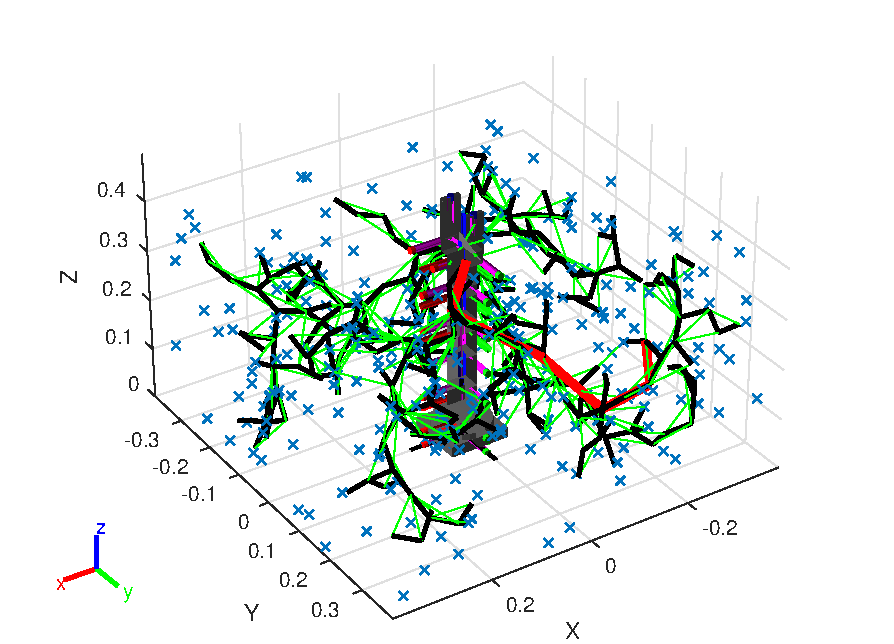
\includegraphics[width = \picsSiz\linewidth]{img/rrt3dex.eps}
        \caption{Result of the RRT algorithm}
        \label{fig:rrt3dex}
    \end{subfigure}
    ~ 
    \begin{subfigure}[htbp]{0.45\textwidth}
        \centering
        \includegraphics[width = \picsSiz\linewidth]{img/rrtSpline.eps}
        \caption{A spline is found based on the results}
        \label{fig:rrtSpline}
    \end{subfigure}
    \caption{3D example of the RRT algoritm}
    \label{fig:rrtsuper}
\end{figure*}
 As one can see in \figref{fig:rrt3dex} there are some green lines. These lines can be seen as shortcuts between each node the length of these shortcuts can be changed. In \figref{fig:rrtSpline} we have a path that is more complicated than it should be and one should maybe consider to increase the length of the shortcuts to get less nodes. These can help to choose less nodes if that is wanted.
 
 \subsubsection{Obstacle avoidance}
 There is no point in doing the RRT if one does not have an obstacle. When an obstacle is added to the search space one have to check if the line connecting the new node to its parent node does not intersect with the object. 
